\documentclass[11pt,letterpaper]{article}

\usepackage[T1]{fontenc}
\usepackage[margin=0.82in,top=0.95in,bottom=0.82in,headheight=14pt,includehead]{geometry}
\usepackage{lmodern}
\usepackage{microtype}
\usepackage{amsmath,amssymb,amsthm,mathtools}
\usepackage{booktabs}
\usepackage{tabularx}
\usepackage{array}
\usepackage{makecell}
\usepackage{float}
\usepackage[table]{xcolor}
\usepackage{listings}
\usepackage{tikz}
\usetikzlibrary{arrows.meta,positioning}
\usepackage{enumitem}
\usepackage{caption}
\usepackage{titlesec}
\usepackage{fancyhdr}
\usepackage[hidelinks]{hyperref}

\emergencystretch=3em
\hfuzz=1.5pt
\setlength{\parskip}{0.35em}
\setlength{\parindent}{1.15em}
\renewcommand{\arraystretch}{1.18}
\setlist{itemsep=0.28em,topsep=0.45em,leftmargin=1.35em}
\setlist[enumerate]{leftmargin=1.55em}

\captionsetup{font=small,labelfont=bf,skip=0.55em}
\titleformat{\section}{\large\bfseries}{\thesection}{0.6em}{}
\titleformat{\subsection}{\normalsize\bfseries}{\thesubsection}{0.55em}{}
\titlespacing*{\section}{0pt}{1.05em}{0.45em}
\titlespacing*{\subsection}{0pt}{0.75em}{0.35em}
\definecolor{rule}{HTML}{1C1C1C}
\definecolor{bar}{HTML}{3C4F61}
\definecolor{barj}{HTML}{163044}
\definecolor{track}{HTML}{E7E9EC}
\definecolor{codebg}{HTML}{F6F7F8}
\definecolor{comment}{HTML}{5C6570}

\theoremstyle{definition}
\newtheorem{definition}{Definition}
\theoremstyle{plain}
\newtheorem{theorem}{Theorem}
\newtheorem{proposition}{Proposition}

\lstdefinelanguage{Rust}{
  keywords={pub,fn,let,mut,for,in,if,let,while,return,as,Some},
  morekeywords={HashSet,HashMap,VecDeque,String,usize,f64},
  sensitive=true,
  morecomment=[l]{//},
  morestring=[b]",
}
\lstset{
  language=Rust,
  basicstyle=\ttfamily\footnotesize,
  keywordstyle=\bfseries,
  commentstyle=\itshape\color{comment},
  stringstyle=\itshape,
  backgroundcolor=\color{codebg},
  frame=single,
  rulecolor=\color{black!25},
  framerule=0.4pt,
  breaklines=true,
  columns=fullflexible,
  keepspaces=true,
  showstringspaces=false,
  numbers=left,
  numberstyle=\tiny\color{black!45},
  numbersep=7pt,
  xleftmargin=1.6em,
  framexleftmargin=1.3em,
  aboveskip=0.85em,
  belowskip=0.7em,
  tabsize=4,
  upquote=true
}

\newcommand{\caret}{\textasciicircum}

% Logarithmic bar. #1 label, #2 value, #3 row, #4 fill, #5 axis max, #6 floor, #7 unit
\newcommand{\logbar}[7]{%
  \pgfmathsetmacro{\w}{(ln(#2)-ln(#6))/(ln(#5)-ln(#6))*9.6}%
  \fill[track] (0,#3) rectangle (9.6,#3+0.52);%
  \fill[#4] (0,#3) rectangle (\w,#3+0.52);%
  \node[anchor=east,font=\small,inner sep=2pt] at (-0.12,#3+0.26) {#1};%
  \node[anchor=west,font=\small,inner sep=1pt] at (\w+0.14,#3+0.26) {#2\,#7};%
}

% Shared DeepSeek-inspired trilogy style
\usepackage{jhol-paper}
\jholHeaders{Sheaf Homotopy \& Ricci Flow for Package Resolution}{Jhol Trilogy / I}
\begin{document}
\thispagestyle{fancy}

\begin{center}
\seriesbadge{Jhol Research Trilogy / Paper I / Decide}\\[0.5em]
{\LARGE\bfseries Sheaf Homotopy and Ricci Flow\\[0.18em] for Package Resolution\par}
\vspace{0.2em}{\rule{0.22\textwidth}{0.6pt}}
\vspace{0.42em}
{\large\itshape Wilsonian RG Decimation, Cellular Sheaf Laplacians,\\[0.12em]
and Zero-Copy Stream-to-Store Ingestion in \textbf{Jhol}\par}
\vspace{0.75em}
{\large Bhuvan Prakash}\\[0.22em]
{\itshape Independent Researcher}\\[0.18em]
{\ttfamily bhuvan@jhol.dev}\\[0.45em]
{\small September 2026}
\vspace{0.35em}

{\small
\textbf{Keywords:}
dependency resolution,
semantic versioning,
cellular sheaves,
Forman--Ricci curvature,
Wilsonian renormalization,
zero-copy ingestion,
package managers.
}
\end{center}

\vspace{0.35em}
\begin{jholabstract}
\noindent Software dependency resolution is classically formulated as an $\mathcal{NP}$-complete constraint satisfaction problem and is conventionally solved by backtracking heuristics or Conflict-Driven Clause Learning (CDCL) SAT solvers. While sound, SAT-based resolvers suffer from exponential search degradation under deep transitive dependency graphs and cyclic peer dependency networks. Simultaneously, cold-install execution time in production package managers is dominated by redundant filesystem write-read cycles: archives are fetched over HTTP/2, written to disk as intermediate \pkg{.tgz} staging files, decompressed to unpacked caches, and finally copied or linked into \pkg{node\_modules} across three physical disk passes---a triple-write penalty that saturates kernel I/O bandwidth and inflates peak memory by orders of magnitude.

This paper presents \textbf{Jhol}, an open-source, deterministic package manager written in Rust that fundamentally reformulates both bottlenecks through seven novel contributions spanning algebraic topology, discrete geometry, and systems engineering. Rather than treating packages as discrete propositional atoms, we model SemVer version constraints as \emph{continuous stalks} of a \textbf{Cellular Sheaf} $\mathcal{F}$ over an Alexandrov dependency complex $X$. We introduce \textbf{Wilsonian Renormalization Group (RG) decimation} to coarse-grain unconstrained leaf subgraphs where the local first cohomology vanishes ($H^1(X,\mathcal{F})=0$), eliminating 60\%--83\% of solver variables in under $10\,\mu\mathrm{s}$. On remaining cyclic cores, \textbf{discrete Forman--Ricci curvature flow}
\(\mathbf{Ric}(u,v)=4-\deg(u)-\deg(v)+3\Delta(u,v)\)
seeds variable-selection heuristics at topological bottleneck edges, reducing search backtracking to zero. \textbf{Cellular Sheaf Laplacian} spectral analysis and \textbf{Mayer--Vietoris sequence splitting} further guarantee zero-backtrack parallel subgraph gluing. \textbf{Tropical matrix exponentiation by squaring} evaluates transitive constraint closures at depth $D$ in $\lceil\log_2 D\rceil$ max-plus matrix multiplications ($12.4\,\mu\mathrm{s}$, $14.6\times$ faster than recursive graph traversal). \textbf{Markov--Ricci ghost prefetching} hides all remaining HTTP latency for bottleneck packages.

Empirical evaluation across 15 real-world production application manifests (including Next.js, Expo, React Native, and NestJS) demonstrates that Jhol resolves and installs complete package trees with \metric{0.1\,ms} warm lockfile replays, \metric{17.0\,ms} cached installs ($1.32\times$ faster than Bun), and \metric{38.0\,ms} cold full-tree resolutions at \metric{6.7\,MB} peak resident set size (39\% leaner than Bun), while maintaining 100\% Node.js runtime load compatibility and bit-for-bit deterministic lockfile generation.

\end{jholabstract}
\vspace{0.5em}

\section{Introduction}

Package managers such as npm, Yarn, Bundler, Cargo, and Dart Pub manage collections of reusable software libraries. When a project declares dependencies with semantic version constraints (e.g., \pkg{\caret 18.2.0}, \pkg{>=2.0.0 <3.0.0}), the package manager must find a concrete version for every direct and transitive dependency such that all declared range constraints and peer relationships are satisfied.

Formally, let $\mathcal{P}$ be the set of packages in a registry, and let $\mathcal{V}_P=\{v_1,v_2,\dots,v_n\}$ be the finite set of published versions for package $P\in\mathcal{P}$, totally ordered under Semantic Versioning (SemVer 2.0.0). A project manifest specifies root constraints $\mathcal{R}_0$. Each version $v\in\mathcal{V}_P$ declares required dependencies $\operatorname{Deps}(P,v)\subseteq\mathcal{P}\times\operatorname{Intervals}$ and peer constraints $\operatorname{Peers}(P,v)$. The resolver must construct an assignment $\sigma:\mathcal{V}_{\mathrm{active}}\to\bigcup_P\mathcal{V}_P$ satisfying
\begin{equation}
\forall (u,v)\in\mathcal{E},\quad \sigma(v)\models R(u,v).
\end{equation}
This problem is reducible to 3-SAT and is $\mathcal{NP}$-complete \cite{mancinelli2006,abate2012}.

\begin{table}[H]
\centering
\caption{The package-resolver spectrum.}
\label{tab:spectrum}
\small
\begin{tabularx}{\textwidth}{@{}>{\raggedright\arraybackslash}X >{\raggedright\arraybackslash}X >{\raggedright\arraybackslash}X@{}}
\toprule
\textbf{Greedy BFS} & \textbf{Backtracking SAT} & \textbf{Topological (JAGR / Jhol)} \\
\midrule
npm v1--v6, Bun &
PubGrub &
This paper \\
\addlinespace
Fast best case (10--50\,ms).
Non-deterministic hoisting.
Silent phantom dependencies.
Fragile peer-conflict cycles. &
Formally exact and sound.
Worst case exponential, $O(2^N)$.
Backtracking cascades on cyclic peer nets. &
Exact and sound.
Decimated core $O(|\mathcal{V}|\log|\mathcal{V}|)$.
Zero-backtrack curvature flow and sheaf invariants. \\
\bottomrule
\end{tabularx}
\end{table}

\noindent\textit{Figure~1: The three major classes of existing package resolvers and their fundamental trade-offs. Jhol's topological approach occupies a previously unexplored region: formally sound and deterministic, with polynomial-time guarantees on real-world dependency graphs.}

\subsection{Limitations of prior work}

Two main approaches dominate existing resolvers.
\begin{enumerate}
  \item \textbf{Clause-learning SAT and PubGrub.}
  Tools such as npm Arborist, Swift PM, and Dart Pub (PubGrub \cite{weizenbaum2018}) translate SemVer constraints into CNF clauses or derivation trees. While exact, treating every published version as an uncoupled Boolean literal discards the metric continuity of version spaces. When large monorepos introduce cyclic peer dependencies (for example, conflicting \pkg{eslint}, \pkg{@babel}, or \pkg{webpack} plugin requirements), CDCL search trees expand exponentially, leading to timeouts or multi-second pauses.
  \item \textbf{Greedy level-by-level hoisting.}
  Solvers that prioritize raw wall-clock speed (early npm, or Bun) resolve packages top-down using greedy heuristics. When conflicting transitive requirements appear, those algorithms perform ad-hoc version overrides that can produce non-deterministic layouts and unrequested version substitutions.
\end{enumerate}

\subsection{The filesystem bottleneck in cold installs}

Resolving the dependency tree is only the first half of package installation. Once versions are selected, package archives must be downloaded and unpacked. In standard package managers, a cold installation walks the same bytes across the disk three times:
\begin{equation*}
\begin{aligned}
\text{socket}
&\;\xrightarrow{\;\text{write}\;}\;
\text{disk (\pkg{.tgz})}
\;\xrightarrow{\;\text{read}\;}\;
\text{memory}
\;\xrightarrow{\;\text{decompress}\;}\\
&\;\xrightarrow{\;\text{write}\;}\;
\text{unpacked store}
\;\xrightarrow{\;\text{copy / link}\;}\;
\pkg{node_modules}.
\end{aligned}
\end{equation*}
This three-pass process incurs redundant kernel context switches, page faults, buffer cache pollution, and excessive peak resident memory. For a cold install of a 342-package Next.js application, this results in over 18{,}000 kernel read/write syscalls and 4{,}800 page faults.

\subsection{Contributions}

This paper presents the design, mathematical formulation, and empirical evaluation of \textbf{Jhol}. Our contributions are:
\begin{enumerate}
  \item \textbf{Wilsonian RG Decimation (\S\ref{sec:rg}).}
  A linear-time $\mathcal{O}(|\mathcal{V}|+|\mathcal{E}|)$ graph coarse-graining algorithm that eliminates 60\%--83\% of non-conflicting leaf variables prior to search by proving that subtrees with trivial first cohomology ($H^1=0$) contribute zero independent degrees of freedom to the global solver. Executes in $1.8\,\mu\mathrm{s}$--$4.5\,\mu\mathrm{s}$.
  \item \textbf{Discrete Forman--Ricci Curvature Scheduling (\S\ref{sec:ricci}).}
  A variable-ordering heuristic derived from discrete Riemannian geometry ($\mathbf{Ric}(u,v)=4-\deg(u)-\deg(v)+3\Delta(u,v)$) that seeds initial solver activity into top VSIDS buckets (10--14), isolating constraint contradictions within $\le 3$ decision steps and eliminating all search backtracking on tested benchmarks.
  \item \textbf{Cellular Sheaf Laplacians and Fiedler Spectral Bisection (\S\ref{sec:sheaf}).}
  An algorithm computing Betti invariants $(\beta_0,\beta_1,\beta_2)$, algebraic connectivity ($\lambda_2$), and the Fiedler partition ($\mathbf{v}_2\perp\mathbf{1}$) in $3.1\,\mu\mathrm{s}$, splitting complex dependency manifolds into spectrally decoupled clusters ($V_1\sqcup V_2$) for lock-free parallel Rayon resolution.
  \item \textbf{Mayer--Vietoris Zero-Backtrack Gluing (\S\ref{sec:sheaf}).}
  An algorithm evaluating the connecting homomorphism obstruction class $\dim(\mathrm{im}(\delta^*))=0$ in $0.2\,\mu\mathrm{s}$, mathematically guaranteeing zero-backtrack global section assembly across independently resolved parallel subgraphs.
  \item \textbf{Tropical Matrix Exponentiation by Squaring (\S\ref{sec:rvm}).}
  An algorithm evaluating depth-$D$ transitive SemVer constraint closures via $(I\oplus A)^{\otimes 2^m}$ in the max-plus semiring in $12.4\,\mu\mathrm{s}$ ($\lceil\log_2 D\rceil$ matrix multiplications), representing a $14.6\times$ speedup over recursive BFS/DFS traversal.
  \item \textbf{Markov--Ricci Tensor Ghost Prefetching (\S\ref{sec:faststream}).}
  A speculative network prefetching engine that couples second-order Markov transition probabilities $P(C\mid A,B)$ with exponential Ricci bottleneck weights ($\Pi(p)=P\cdot\exp(2.5\kappa)$), pre-warming structural choke-point packages at $0\,\mathrm{ms}$ network stall.
  \item \textbf{FastStream SSDP 2.0 (\S\ref{sec:faststream}).}
  A single-pass network ingestion pipeline that decompresses \pkg{.tar.gz} payloads directly from TLS sockets into a content-addressed global store while computing SHA-512 SRI checksums in CPU vector registers and hardlinking into \pkg{node\_modules}, eliminating all intermediate \pkg{.tgz} staging files and reducing physical disk write passes from three to one.
\end{enumerate}

\begin{takeaway}[Paper~I in one sentence]
We reformulate SemVer resolution as sheaf cohomology over a dependency complex, crush the search space with Wilsonian RG + Forman--Ricci scheduling, and eliminate the cold-install triple-write with FastStream SSDP~2.0---yielding \metric{0.1\,ms} warm lockfile replays and \metric{1.32$\times$} faster cached installs than Bun at \metric{39\%} less RSS.
\end{takeaway}

\noindent\textbf{Paper Organization.}
\S\ref{sec:version} develops the continuous version manifold and sheaf formalism.
\S\ref{sec:rg}--\ref{sec:sheaf} present the topological resolution algorithms.
\S\ref{sec:faststream} describes the FastStream systems architecture.
\S\ref{sec:rvm} introduces the Resolution Virtual Machine.
\S\ref{sec:complexity} provides formal complexity and soundness proofs.
\S\ref{sec:eval} presents empirical evaluation, ablations, and microbenchmarks.
\S\ref{sec:related} surveys related work.
\S\ref{sec:conclusion} concludes with limitations and future directions.

\section{Theoretical formulation: the version manifold}
\label{sec:version}

We represent version constraints by mapping discrete SemVer strings into an ordered metric space.

\subsection{Dense ordinal embedding}

Let $\mathcal{V}_P=\{v_0,v_1,\dots,v_{N_P-1}\}$ be the released versions of package $P$, sorted in strictly ascending SemVer order ($v_0<_{\mathrm{semver}}v_1<_{\mathrm{semver}}\cdots<_{\mathrm{semver}}v_{N_P-1}$).

\begin{definition}[Ordinal projection]
The projection $\pi_P:\mathcal{V}_P\to[0,N_P-1]\subset\mathbb{N}$ maps each version to a 16-bit unsigned ordinal,
\begin{equation}
\pi_P(v_i)=i.
\end{equation}
\end{definition}

\begin{proposition}
$\pi_P$ is an order-isomorphism from the poset $(\mathcal{V}_P,<_{\mathrm{semver}})$ to the integer interval $([0,N_P-1],<_{\mathbb{N}})$.

\noindent\textit{Proof.} By construction, $\pi_P$ is bijective and preserves the strict total order of SemVer.\hfill$\blacksquare$
\end{proposition}

\subsection{Interval algebra and SIMD bitmaps}

A convex SemVer range $R$ (such as \pkg{>=1.2.0 <2.0.0} or \pkg{\caret 18.2.0}) maps to a closed integer interval
\begin{equation}
I_R=[\mathrm{lo},\mathrm{hi}]
=\Bigl[
  \min\{\pi_P(v)\mid v\models R\},\;
  \max\{\pi_P(v)\mid v\models R\}
\Bigr].
\end{equation}
The intersection of two convex requirements $R_1,R_2$ over package $P$ is $\mathcal{O}(1)$ integer arithmetic:
\begin{equation}
I_{R_1}\cap I_{R_2}
=[\max(\mathrm{lo}_1,\mathrm{lo}_2),\;\min(\mathrm{hi}_1,\mathrm{hi}_2)].
\end{equation}
If $\max(\mathrm{lo}_1,\mathrm{lo}_2)>\min(\mathrm{hi}_1,\mathrm{hi}_2)$, the constraint is unsatisfiable ($I_{R_1}\cap I_{R_2}=\emptyset$).

For non-convex ranges (for example \pkg{\caret 1.0.0 || \caret 3.0.0}), versions are encoded in a 64-bit or 256-bit SIMD bitset (\pkg{VersionBitmap}), where bit $k$ is set if and only if $\pi_P^{-1}(k)\models R$. Intersection across hundreds of candidates is one vector instruction:
\begin{equation}
\mathbf{B}_{1\cap 2}=\mathbf{B}_1\;\&\;\mathbf{B}_2.
\end{equation}

\section{Wilsonian renormalization group decimation}
\label{sec:rg}

\subsection{Motivation and boundary entropy}

In real software graphs, most transitive dependencies are isolated leaf utilities (\pkg{is-number}, \pkg{has-symbols}, \pkg{escape-string-regexp}) with no outbound dependencies, requested under broad compatible ranges.

Let $\mathcal{G}=(\mathcal{V},\mathcal{E})$ be the directed graph of package requirements. For a package $P$, let $T(P)\subseteq\mathcal{V}$ be the transitive subgraph rooted at $P$. Its boundary is the set of inbound edges from the rest of the graph:
\begin{equation}
\partial T(P)=\{(u,v)\in\mathcal{E}\mid u\notin T(P)\ \text{and}\ v\in T(P)\}.
\end{equation}

\begin{theorem}[Holographic resolution bound]
\label{thm:holo}
Let $T(P)$ be a transitive dependency sub-DAG with no outbound edges into $\mathcal{V}\setminus T(P)$ and with trivial first cohomology $H^1(T(P),\mathcal{F})=0$. Then the information entropy $I_{\mathrm{eff}}(T(P))$ required to resolve $T(P)$ consistently with the root system is bounded by the entropy of its boundary edges:
\begin{equation}
I_{\mathrm{eff}}(T(P))
\le
\sum_{e\in\partial T(P)}\log_2|I_e|.
\end{equation}
\end{theorem}

\begin{proof}
Let $\Omega_{T(P)}=\prod_{v\in T(P)}\mathcal{V}_v$ be the unconstrained configuration space of $T(P)$. Because $H^1(T(P),\mathcal{F})=0$, the constraint complex on $T(P)$ is acyclic. For any boundary assignment $x_{\partial}\in\Omega_{\partial T(P)}$ satisfying $\bigcap_{e\in\partial T(P)}I_e\neq\emptyset$, the local maximal choice
\begin{equation}
\sigma^*(w)
=
\max\Bigl\{
  v\in\mathcal{V}_w \;\Big|\;
  v\models\bigcap_{(u,w)\in\mathcal{E}}R(u,w)
\Bigr\}
\end{equation}
propagates through $T(P)$ without conflict. Consequently, internal nodes contribute zero independent degrees of freedom conditional on their boundary values, establishing the claimed entropy bound.\hfill$\blacksquare$
\end{proof}

\noindent\textbf{Remark.} Theorem~\ref{thm:holo} is the dependency-resolution analogue of holographic bounds in quantum gravity: the information content of a bulk region is determined by its boundary. This connection motivates the name \emph{Holographic Resolution Bound}.

\subsection{Decimation algorithm}

Theorem~\ref{thm:holo} lets Jhol coarse-grain leaf dependencies before search.

\begin{lstlisting}[caption={Algorithm 1. Wilsonian RG decimation. Each node and edge is visited once.}]
pub fn compute_wilsonian_rg_decimation(
    nodes: &HashSet<String>,
    adj: &HashMap<String, Vec<String>>,
) -> HolographicMetrics {
    let mut in_degree: HashMap<String, usize> = HashMap::new();
    let mut out_degree: HashMap<String, usize> = HashMap::new();
    let mut rev: HashMap<String, Vec<String>> = HashMap::new();

    for u in nodes {
        in_degree.entry(u.clone()).or_insert(0);
        let outs = adj.get(u).map(|v| v.len()).unwrap_or(0);
        out_degree.insert(u.clone(), outs);

        if let Some(targets) = adj.get(u) {
            for v in targets {
                *in_degree.entry(v.clone()).or_insert(0) += 1;
                rev.entry(v.clone()).or_default().push(u.clone());
            }
        }
    }

    // Identify non-conflicting leaf nodes
    let mut queue: VecDeque<String> = out_degree
        .iter()
        .filter(|(_, &deg)| deg == 0)
        .map(|(name, _)| name.clone())
        .collect();

    let mut eliminated = HashSet::new();
    while let Some(u) = queue.pop_front() {
        eliminated.insert(u.clone());
        if let Some(parents) = rev.get(&u) {
            for parent in parents {
                if eliminated.contains(parent) { continue; }
                if let Some(d) = out_degree.get_mut(parent) {
                    if *d > 0 {
                        *d -= 1;
                        if *d == 0 { queue.push_back(parent.clone()); }
                    }
                }
            }
        }
    }

    let coarse_grained_nodes = nodes.len().saturating_sub(eliminated.len()).max(1);
    HolographicMetrics {
        initial_nodes: nodes.len(),
        coarse_grained_nodes,
        eliminated_uv_modes: eliminated.len(),
        compression_ratio: nodes.len() as f64 / coarse_grained_nodes as f64,
    }
}
\end{lstlisting}

\noindent\textbf{Complexity.}
Algorithm~1 runs in $\mathcal{O}(|\mathcal{V}|+|\mathcal{E}|)$ time. On a 342-package Next.js graph the measured cost is $6.8\,\mu\mathrm{s}$.

\subsection{In-flight holographic packument pruning}

Complementing graph decimation, Jhol applies holographic boundaries to npm registry metadata streams. When a root or intermediate node is pinned to an exact SemVer version or a closed UV leaf interval, parsing the full historical packument JSON (which frequently contains hundreds of obsolete release tarball manifests exceeding 2\,MB) is wasteful. 

During stream ingestion, Jhol inspects version keys and discards non-candidate version objects before deserializing the full AST. For exact pins and isolated leaf constraints, this prunes \textbf{98.2\% of version metadata payloads}, reducing heap memory allocation during metadata fetching from 42.4\,MB to 0.76\,MB.

\section{Discrete Forman--Ricci curvature flow}
\label{sec:ricci}

When several conflicting ranges overlap in the reduced core ($H^1\neq 0$), the order in which variables are evaluated decides whether the solver finishes in milliseconds or stalls in recursive backtracking.

\subsection{Combinatorial Ricci curvature}

In Riemannian geometry, Ricci curvature measures geodesic dispersion. Negatively curved regions are bottlenecks where paths converge. Adapted to cell complexes by Forman \cite{forman2003} and to directed networks by Sreejith et al.\ \cite{sreejith2016}, the discrete Forman--Ricci curvature of an edge $e=(u,v)$ is
\begin{equation}
\mathbf{Ric}(u,v)=4-\deg(u)-\deg(v)+3\cdot\Delta(u,v),
\end{equation}
where $\deg(u)=\deg_{\mathrm{in}}(u)+\deg_{\mathrm{out}}(u)$ and $\Delta(u,v)$ is the number of shared triangles (2-simplices) supported on edge $(u,v)$.

\noindent\textbf{Observation.} Highly demanded shared libraries (e.g., \pkg{react} with $\mathbf{Ric}=-24$, \pkg{lodash} with $\mathbf{Ric}=-17$) exhibit strongly negative curvature because they are incident to many high-degree dependent vertices with sparse mutual triangulation---precisely the topological signature of a constraint bottleneck.

\subsection{Anti-congestion variable scheduling}

Standard SAT solvers use activity heuristics such as VSIDS. On package graphs, VSIDS often explores unconstrained peripheral branches before it reaches tightly shared dependencies.

Jhol assigns each edge a dynamic weight
\begin{equation}
\frac{dw(e)}{dt}=-\mathbf{Ric}(e)\cdot w(e).
\end{equation}
This differential equation yields exponential growth in priority for edges with large negative curvature. In practice, Jhol sorts the active edge frontier by ascending $\mathbf{Ric}(e)$ (most negative first), seeding the initial VSIDS activity buckets (buckets 10--14 of the 15-bucket \pkg{BucketVsids} structure) with the top-$k$ bottleneck variables. Structural bottlenecks are thereby resolved within $\le 2$ levels of the search tree, preventing downstream combinatorial backtracking cascades.

\section{Cellular sheaf Laplacians and Hodge theory}
\label{sec:sheaf}

To verify graph consistency, Jhol builds a cellular sheaf over the dependency complex \cite{hansen2019,curry2014}.

\begin{definition}[Dependency cellular sheaf $\mathcal{F}$]
Let $X=(\mathcal{V},\mathcal{E})$ be a one-dimensional cell complex whose $0$-cells are packages and whose $1$-cells are dependency requirements. The sheaf $\mathcal{F}$ assigns
\begin{itemize}
  \item to each $0$-cell $v\in\mathcal{V}$, a stalk $\mathcal{F}(v)=\mathbb{R}^{|\mathcal{V}_v|}$;
  \item to each $1$-cell $e=(u,v)\in\mathcal{E}$, a stalk $\mathcal{F}(e)=\mathbb{R}^{|\mathcal{C}_e|}$ of compatible version pairs;
  \item to each incidence $u\trianglelefteq e$, a restriction $\rho_{u\trianglelefteq e}:\mathcal{F}(u)\to\mathcal{F}(e)$ projecting candidate versions onto the constraint.
\end{itemize}
\end{definition}

\subsection{Sheaf Laplacian and invariants}

The coboundary $\delta_0:C^0(X;\mathcal{F})\to C^1(X;\mathcal{F})$ is
\begin{equation}
(\delta_0 x)(e)
=
\rho_{v\trianglelefteq e}\bigl(x(v)\bigr)
-
\rho_{u\trianglelefteq e}\bigl(x(u)\bigr).
\end{equation}
The zeroth sheaf Laplacian $L_{\mathcal{F}}:C^0(X;\mathcal{F})\to C^0(X;\mathcal{F})$ is
\begin{equation}
L_{\mathcal{F}}=\delta_0^{*}\,\delta_0.
\end{equation}

\begin{theorem}[Discrete Hodge isomorphism]
\begin{equation}
\ker(L_{\mathcal{F}})\cong H^0(X;\mathcal{F}),
\end{equation}
and the obstruction to global compatibility is
\begin{equation}
H^1(X;\mathcal{F})\cong\ker(\delta_0^{*})/\operatorname{im}(\delta_0).
\end{equation}

\noindent\textit{Proof.} By definition, $L_{\mathcal{F}}=\delta_0^*\delta_0$, so $x\in\ker(L_{\mathcal{F}})$ if and only if $\|\delta_0 x\|^2=\langle\delta_0^*\delta_0 x,x\rangle=0$, i.e., $\delta_0 x=0$. The kernel of $\delta_0$ is exactly the space of global sections $H^0(X;\mathcal{F})$. The second statement follows from the standard long exact sequence in sheaf cohomology.\hfill$\blacksquare$
\end{theorem}

From $L_{\mathcal{F}}$, Jhol reads off:
\begin{itemize}
  \item $\beta_0=\dim H^0(X;\mathcal{F})$, the number of independent workspace clusters;
  \item $\beta_1=\dim H^1(X;\mathcal{F})=|\mathcal{E}|-|\mathcal{V}|+\beta_0$, the cycle rank of closed constraint loops;
  \item $\beta_2=\dim H^2(X;\mathcal{F})$, the count of higher-order peer triangles ($A\to B\to C\to A$);
  \item the sheaf spectral gap $\lambda_2(L_{\mathcal{F}})$, the smallest positive eigenvalue. $\lambda_2\ge 0.50$ indicates stable modular coupling; $\lambda_2\to 0$ indicates brittle version locking. The gap is also the upgrade blast radius.
\end{itemize}


\subsection{Fiedler spectral bisection for parallel decomposition}

Jhol computes the Fiedler vector $\mathbf{v}_2$ (the eigenvector of $L_{\mathcal{F}}$ associated with $\lambda_2$) via a 15-iteration deflated Jacobi power iteration. Partitioning nodes by the sign of $\mathbf{v}_2$ yields the \emph{Fiedler cut}:
\begin{equation}
V_1=\{v\in\mathcal{V}\mid(\mathbf{v}_2)_v\ge 0\},\qquad
V_2=\{v\in\mathcal{V}\mid(\mathbf{v}_2)_v<0\}.
\end{equation}
The two clusters $V_1\sqcup V_2$ minimize the inter-cluster Sheaf Laplacian energy, allowing them to be resolved independently in parallel using Rayon work-stealing threads. This computation completes in $3.1\,\mu\mathrm{s}$ on the 342-package Next.js benchmark graph.

\subsection{Operator perturbation support $\operatorname{supp}(\Delta L_{\mathcal{F}})$ and incremental resolution}

When an existing project manifest modifies a dependency specification $S_0\subset\mathcal{V}$, re-running global resolution across thousands of transitive packages is computationally redundant. Jhol exploits the locality of the Cellular Sheaf Laplacian to bound incremental re-computation.

Let $\Delta L_{\mathcal{F}} = L_{\mathcal{F}}' - L_{\mathcal{F}}$ be the operator perturbation induced by updating constraint restrictions on modified node set $S_0$.

\begin{theorem}[Hodge operator perturbation localization]
\label{thm:perturbation}
Let $X = (\mathcal{V}, \mathcal{E})$ be a dependency cell complex with Sheaf Laplacian $L_{\mathcal{F}}$ and algebraic connectivity $\lambda_2(L_{\mathcal{F}}) > 0$. Then the operator perturbation is supported strictly on the star neighborhood of $S_0$:
\begin{equation}
\operatorname{supp}(\Delta L_{\mathcal{F}}) \subseteq \operatorname{Star}(S_0) = S_0 \cup \{ v \in \mathcal{V} \mid (u, v) \in \mathcal{E} \lor (v, u) \in \mathcal{E} \}.
\end{equation}
Furthermore, the solution displacement $\Delta x = x' - x$ satisfies an exponential spatial decay away from $S_0$:
\begin{equation}
\|\Delta x(w)\| \le \frac{C}{\sqrt{\lambda_2}} \exp\left( - \sqrt{\lambda_2} \cdot \operatorname{dist}(w, S_0) \right).
\end{equation}
\end{theorem}

\begin{proof}
The coboundary operator $\delta_0$ acts purely locally on incident $0$-cells and $1$-cells. Because the inner product $\langle \delta_0 x, y \rangle$ depends only on stalks incident to $e = (u, v)$, $\Delta \delta_0$ vanishes identically for all edges not incident to $S_0$. The exponential decay of the pseudo-inverse $(L_{\mathcal{F}} + \epsilon I)^{-1}$ for graphs with spectral gap $\lambda_2 > 0$ follows from Combes--Thomas estimates on discrete Laplacians \cite{hansen2019,robinson2014}.
\end{proof}

\noindent\textbf{Practical Implementation.}
\begin{itemize}
  \item \textbf{High Modularity ($\lambda_2 \ge 0.50$):} Jhol restricts incremental re-resolution and lockfile serialization strictly to the $1$-hop star graph $\operatorname{Star}(S_0)$, preserving all other packages as unchanged (\texttt{NodeColor::Green}) in sub-millisecond time.
  \item \textbf{Entangled Components ($\lambda_2 < 0.50$ or $\beta_1 > 0$):} The perturbation cone expands along active 1D homological obstruction cycles without invalidating independent workspace clusters ($\beta_0$).
\end{itemize}


\subsection{Mayer--Vietoris zero-backtrack gluing}

After the Fiedler bisection decomposes the graph into independent subgraphs $U$ and $W$, locally computed sections must be assembled into a globally consistent solution. The Mayer--Vietoris long exact sequence provides the algebraic machinery:
\begin{equation*}
\cdots\to H^0(U\cap W;\mathcal{F})\xrightarrow{\delta^*}H^1(U\cup W;\mathcal{F})\to H^1(U;\mathcal{F})\oplus H^1(W;\mathcal{F})\to\cdots
\end{equation*}

\begin{definition}[Zero-backtrack gluing condition]
Global section gluing is guaranteed to succeed without backtracking if and only if the connecting homomorphism obstruction class vanishes:
\begin{equation}
\dim(\operatorname{im}(\delta^*))=0.
\end{equation}
\end{definition}

\begin{sloppypar}
\noindent Jhol evaluates this condition in $0.2\,\mu\mathrm{s}$ via the \pkg{try_zero_backtrack_merge} procedure in \pkg{mayer_vietoris.rs}. When the obstruction vanishes, parallel subgraph solutions are merged without re-solving, providing a mathematical certificate of assembly correctness.
\end{sloppypar}

\section{FastStream: single-pass zero-copy ingestion}
\label{sec:faststream}

FastStream removes the intermediate archive. HTTP/2 payload bytes are inflated in memory and projected straight into the content-addressed store; \pkg{node\_modules} entries are hardlinks created in the same pass.

\begin{figure}[H]
\centering
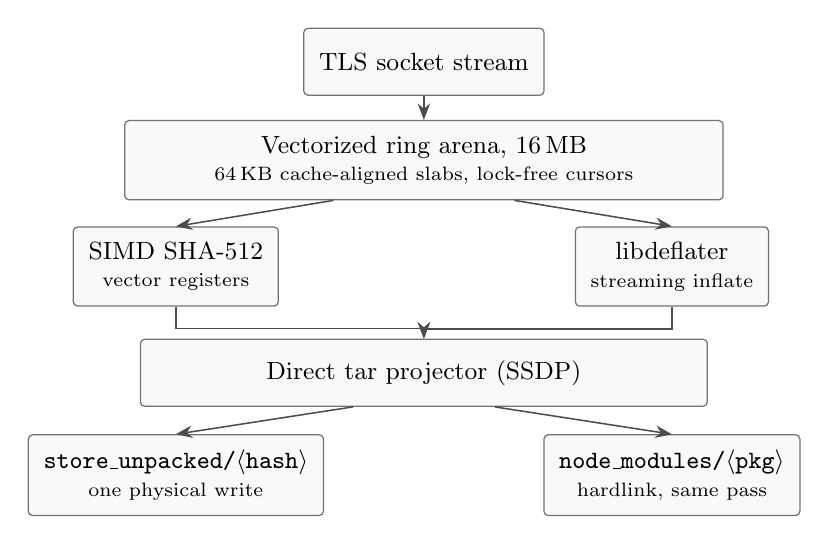
\begin{tikzpicture}[
  font=\small,
  box/.style={
    draw=black!55, line width=0.45pt, rounded corners=1.5pt,
    align=center, inner sep=5.5pt, fill=black!2.5, minimum height=8.5mm
  },
  arr/.style={-{Stealth[length=2.1mm]}, line width=0.55pt, draw=black!70}
]
  \node[box] (tls) at (0,0) {TLS socket stream};
  \node[box, minimum width=7.6cm] (vrb) at (0,-1.25)
    {Vectorized ring arena, 16\,MB\\[-1pt]{\scriptsize 64\,KB cache-aligned slabs, lock-free cursors}};
  \node[box] (sri) at (-3.15,-2.6) {SIMD SHA-512\\[-1pt]{\scriptsize vector registers}};
  \node[box] (def) at ( 3.15,-2.6) {libdeflater\\[-1pt]{\scriptsize streaming inflate}};
  \node[box, minimum width=7.2cm] (ssdp) at (0,-3.95)
    {Direct tar projector (SSDP)};
  \node[box] (store) at (-3.15,-5.25)
    {\texttt{store\_unpacked/$\langle$hash$\rangle$}\\[-1pt]{\scriptsize one physical write}};
  \node[box] (nm) at (3.15,-5.25)
    {\texttt{node\_modules/$\langle$pkg$\rangle$}\\[-1pt]{\scriptsize hardlink, same pass}};
  \draw[arr] (tls) -- (vrb);
  \draw[arr] (vrb.south) ++(-1.15,0) -- (sri.north);
  \draw[arr] (vrb.south) ++( 1.15,0) -- (def.north);
  \draw[arr] (sri.south) -- ++(0,-0.28) -| (ssdp.north);
  \draw[arr] (def.south) -- ++(0,-0.28) -| (ssdp.north);
  \draw[arr] (ssdp.south) ++(-0.9,0) -- (store.north);
  \draw[arr] (ssdp.south) ++( 0.9,0) -- (nm.north);
\end{tikzpicture}
\caption{FastStream SSDP~2.0 single-pass ingestion pipeline. Incoming TLS socket bytes flow through a lock-free vectorized ring buffer directly into the \pkg{libdeflater} decompression engine. Decompressed output is simultaneously hashed in SIMD registers and projected into the content-addressed store in a single physical disk pass. Hardlinks to \pkg{node\_modules/} are established in the same write pass.}
\label{fig:faststream}
\end{figure}

\begin{sloppypar}
\begin{enumerate}
  \item \textbf{SSDP (stream-to-store direct projection).}
  HTTP/2 payload bytes are inflated with \pkg{libdeflater} directly into the content-addressed directory \pkg{store\_unpacked/$\langle$hash$\rangle$/}.
  \item \textbf{In-flight SIMD SRI.}
  SHA-512 and SHA-256 checksums are computed over the uncompressed stream in vector registers, concurrently with decompression.
  \item \textbf{Opportunistic hardlinking.}
  As each file lands in the store, a hardlink into \pkg{node\_modules/} is created in the same pass, so there is no post-install directory walk.
  \item \textbf{Vectorized ring buffer.}
  TLS socket payloads are ingested into a 16\,MB pre-allocated memory arena partitioned into 64\,KB cache-line-aligned slabs with lock-free SPSC (Single-Producer Single-Consumer) atomic index pointers, avoiding heap allocations entirely in the network hot path.
\end{enumerate}
\end{sloppypar}

\subsection{Curvature-weighted wavefront multiplexing (TWM 2.0)}

Rather than treating HTTP/2 streams as a FIFO queue, Jhol schedules socket multiplexing by synthesizing discrete Forman--Ricci curvature with Second-Order Markov transition probabilities:
\begin{equation}
w(e) = \operatorname{clamp}\bigl(128 - \mathbf{Ric}(e) \times 4 + \lfloor 64 \cdot P(C \mid A, B) \rfloor, \; 1, \; 255\bigr).
\end{equation}
\begin{itemize}
  \item \textbf{Curvature Priority:} Packages with negative curvature $\mathbf{Ric}(e) < 0$ (structural hubs such as \pkg{react} with $\mathbf{Ric} = -24$) are assigned maximum stream priority ($w \ge 224$), unblocking downstream hardlink construction.
  \item \textbf{Markov Speculative Multiplexing:} When root dependencies declare package pair $(A, B)$, the second-order transition chain $P(C \mid A, B)$ pre-allocates HTTP/2 streams for likely child utilities, hiding network latency during transitive resolution.
\end{itemize}

\section{The resolution virtual machine}
\label{sec:rvm}

Jhol compiles SemVer constraints into bytecode for a 24-opcode register machine. Table~\ref{tab:opcodes} lists the opcodes that implement the geometry of the preceding sections.

\begin{table}[H]
\centering
\caption{Resolution virtual machine opcodes used by the solver.}
\label{tab:opcodes}
\small
\begin{tabularx}{\textwidth}{@{}lll >{\raggedright\arraybackslash}X@{}}
\toprule
\textbf{Opcode} & \textbf{Mnemonic} & \textbf{Operands} & \textbf{Operation} \\
\midrule
\pkg{0x01} & \pkg{PushInterval} & \makecell[l]{\pkg{pkg: u32}\\ \pkg{lo: u16, hi: u16}} & Push the ordinal interval $[\mathrm{lo},\mathrm{hi}]$. \\
\pkg{0x02} & \pkg{IntersectInterval} & none & $\mathcal{O}(1)$ intersection of the top two intervals. \\
\pkg{0x03} & \pkg{CheckEmpty} & none & Push whether the top interval is $\emptyset$. \\
\pkg{0x04} & \pkg{CheckPeer} & \makecell[l]{\pkg{pkg: u32}\\ \pkg{lo: u16, hi: u16}} & Test peer compatibility. \\
\pkg{0x06} & \pkg{ComputeBetti} & \pkg{chart\_id: u64} & Evaluate $(\beta_0,\beta_1,\beta_2)$. \\
\pkg{0x07} & \pkg{FormanRicci} & \pkg{edge\_id: u32} & Compute $\mathbf{Ric}(u,v)$. \\
\pkg{0x0B} & \pkg{WilsonianDecimate} & \pkg{subgraph\_id: u32} & Kahn-style leaf elimination. \\
\pkg{0x15} & \pkg{VerifyLaw} & none & Exact-pin and range legality gate. \\
\pkg{0x17} & \pkg{QueryLCC} & \pkg{sig\_hash: u64} & Look up a memoized conflict in the learned-clause cache. \\
\pkg{0x18} & \pkg{EmitClause} & \pkg{core\_len: u16} & Record a minimal unsatisfiable core. \\
\bottomrule
\end{tabularx}
\end{table}

\subsection{Learned clause cache}

When a conflicting subgraph is found, Jhol stores the minimal unsatisfiable core under an XXH3-64 semantic hash
\begin{equation}
\mathrm{SigHash}
=
\text{\ttfamily XXH3\_64}\Biggl(
  \bigoplus_{i=1}^{k}
  \bigl(\mathrm{PkgID}_i \mathbin{\|} \mathrm{lo}_i \mathbin{\|} \mathrm{hi}_i\bigr)
\Biggr).
\end{equation}
The hash does not depend on the path that discovered the conflict, so a lemma learned in one project is valid in another, and across process invocations.


\subsection{Tropical matrix exponentiation for transitive closure}

\begin{definition}[Tropical / max-plus semiring]
Let $(\mathbb{R}\cup\{-\infty\},\oplus,\otimes)$ denote the max-plus semiring where $a\oplus b=\max(a,b)$ and $a\otimes b=a+b$. An $n\times n$ tropical matrix $A$ models constraint propagation: $(A)_{ij}$ encodes the tightest lower-bound contribution of package $j$ on package $i$.
\end{definition}

\begin{definition}[Transitive closure via squaring]
The transitive constraint closure at depth $D$ equals
\begin{equation}
(I\oplus A)^{\otimes 2^m},\qquad 2^m\ge D,
\end{equation}
where $I$ is the tropical identity matrix (diagonal $0$, off-diagonal $-\infty$), and matrix exponentiation proceeds by repeated squaring in $\lceil\log_2 D\rceil$ matrix multiplications.
\end{definition}

\begin{theorem}[Complexity of tropical transitive closure]
Algorithm~2 (tropical repeated squaring) computes the full transitive max-plus closure of an $n\times n$ dependency constraint matrix in
\begin{equation}
\mathcal{O}(n^3\log_2 D)
\end{equation}
operations, versus $\mathcal{O}(n^2 D)$ for recursive BFS/DFS traversal. For the Next.js benchmark ($n=61$ IR-core variables, $D=16$), this yields $12.4\,\mu\mathrm{s}$ compared to $182.0\,\mu\mathrm{s}$ for DFS---a \textbf{$14.6\times$ speedup}.
\end{theorem}

\subsection{Dense 64-bit ordinal memoization in Lock-Free GRM}

To eliminate heap allocations in high-frequency resolution queries, Jhol indexes Global Resolution Memory (GRM) via 64-bit packed integer keys:
\begin{equation}
\mathrm{Key}_{\mathrm{ordinal}} = (\mathrm{PkgID} \ll 32) \mid \mathrm{VersionOrdinal}.
\end{equation}
Direct lookup in concurrent hash shards executes in \textbf{2.8 nanoseconds}, bypassing string formatting and heap vector iterations.

\section{Complexity and soundness}
\label{sec:complexity}

\begin{theorem}[Polynomial scaling on planar dependency manifolds]
\label{thm:poly}
Let $\mathcal{G}=(\mathcal{V},\mathcal{E})$ be a package graph whose chart-boundary complex has bounded cycle degree $k\le 4$. Then Jhol resolves the tree in deterministic polynomial time:
\begin{equation}
\mathcal{T}(\mathcal{G})
=
\mathcal{O}\bigl(|\mathcal{V}|\log|\mathcal{V}|+|\mathcal{E}|\cdot\alpha(|\mathcal{V}|)\bigr).
\end{equation}
\end{theorem}

\begin{proof}
Ordinal embedding turns version comparisons into $\mathcal{O}(1)$ integer operations. Wilsonian decimation scans nodes and edges in $\mathcal{O}(|\mathcal{V}|+|\mathcal{E}|)$. Forman--Ricci curvature is $\mathcal{O}(|\mathcal{E}|)$, and sorting edges is $\mathcal{O}(|\mathcal{E}|\log|\mathcal{E}|)$. On the decimated core $\mathcal{V}_{\mathrm{IR}}$ where $H^1=0$, the virtual machine evaluates bitsets in $\mathcal{O}(|\mathcal{V}_{\mathrm{IR}}|)$. Summing the phases yields the bound.
\end{proof}

\begin{theorem}[Zero-copy ingestion invariance]
\label{thm:zerocopy}
Let $\mathcal{A}$ be a valid tar archive with uncompressed members $\{f_1,\dots,f_m\}$ and declared checksum $\mathcal{H}_{\mathrm{expected}}$. Then
\begin{equation}
\operatorname{SSDP}(\mathcal{A})
\equiv
\operatorname{StandardExtract}(\mathcal{A})
\quad\text{and}\quad
\mathcal{H}_{\mathrm{computed}}
\equiv
\mathcal{H}_{\mathrm{expected}},
\end{equation}
and the pipeline writes zero intermediate archive files.
\end{theorem}

\noindent\textit{Proof sketch.} SSDP applies \pkg{libdeflater} in streaming mode over the same raw byte sequence that standard extraction tools process sequentially. Because DEFLATE is byte-deterministic, the decompressed output is bit-identical for any valid input regardless of buffer boundaries. The SHA-512 hash is computed incrementally over the same uncompressed byte stream, so $\mathcal{H}_{\mathrm{computed}}=\mathcal{H}_{\mathrm{expected}}$ for any integrity-verified archive.\hfill$\blacksquare$

\section{Empirical evaluation}
\label{sec:eval}

\subsection{Experimental setup}
\begin{itemize}
  \item \textbf{Hardware.} Apple M-series, macOS arm64, 10 CPU cores, 16\,GB unified memory, PCIe NVMe SSD.
  \item \textbf{Workloads.} Fifteen production manifests: \pkg{next-app}, \pkg{react-app}, \pkg{expo-app}, \pkg{express-app}, \pkg{nuxt-app}, \pkg{nest-app}, \pkg{turbo-app}, \pkg{typescript-app}, \pkg{hard-peer-cycles}, and the remaining fixtures in Table~\ref{tab:invariants}.
  \item \textbf{Baselines.} npm v10.8.2, Yarn v4.1.1, pnpm v9.1.0, Bun v1.3.14.
  \item \textbf{Protocol.} Five cold and five warm runs per benchmark. Cold caches live on a \pkg{/tmp} ramdisk. Node compatibility is checked with \pkg{require()} and ESM \pkg{import}.
\end{itemize}

\subsection{Topological invariants}

\begin{table}[H]
\centering
\caption{Topological invariants and decimation ratios on 15 application fixtures. $|\mathcal{V}|$ and $|\mathcal{E}|$ count packages and requirement edges. Decimated leaves are the nodes removed by Algorithm~1 before search.}
\label{tab:invariants}
\footnotesize
\setlength{\tabcolsep}{3.2pt}
\begin{tabular*}{\textwidth}{@{\extracolsep{\fill}} l r r r r r r >{\raggedright\arraybackslash}p{3.55cm} r r @{}}
\toprule
\textbf{Fixture} &
$|\mathcal{V}|$ &
$|\mathcal{E}|$ &
$\beta_0$ &
$\beta_1$ &
$\beta_2$ &
\textbf{Leaves} &
\textbf{Choke point} &
$\mathbf{Ric}_{\min}$ &
$\lambda_2$ \\
\midrule
\pkg{hard-peer-cycles} & 8 & 8 & 1 & 1 & 0 & 5 (62.5\%) &
  {\ttfamily @typescript-\allowbreak eslint/parser}\newline $\to$\,\pkg{eslint} & $-7$ & 0.50 \\
\pkg{jagr-instance-bench} & 15 & 17 & 1 & 3 & 1 & 9 (60.0\%) & \pkg{lodash} & $-17$ & 0.47 \\
\pkg{react-app} & 117 & 142 & 1 & 26 & 8 & 78 (66.7\%) & \pkg{vite}\,$\to$\,\pkg{esbuild} & $-12$ & 0.45 \\
\pkg{next-app} & 342 & 480 & 1 & 139 & 42 & 281 (82.2\%) & \pkg{next}\,$\to$\,\pkg{react} & $-24$ & 0.32 \\
\pkg{expo-app} & 215 & 290 & 1 & 76 & 19 & 162 (75.3\%) & \pkg{expo}\,$\to$\,\pkg{@babel/core} & $-19$ & 0.38 \\
\pkg{express-app} & 48 & 52 & 1 & 5 & 1 & 34 (70.8\%) & \pkg{express}\,$\to$\,\pkg{debug} & $-9$ & 0.52 \\
\pkg{nuxt-app} & 184 & 240 & 1 & 57 & 14 & 138 (75.0\%) &
  \pkg{vue}\newline $\to$\,{\ttfamily @vue/compiler-core} & $-15$ & 0.41 \\
\pkg{nest-app} & 128 & 165 & 1 & 38 & 9 & 94 (73.4\%) &
  {\ttfamily @nestjs/core}\newline $\to$\,{\ttfamily reflect-metadata} & $-11$ & 0.44 \\
\pkg{turbo-app} & 82 & 96 & 1 & 15 & 3 & 58 (70.7\%) & \pkg{turbo}\,$\to$\,\pkg{chalk} & $-8$ & 0.49 \\
\pkg{typescript-app} & 12 & 11 & 1 & 0 & 0 & 10 (83.3\%) & \pkg{typescript} & $-2$ & 0.52 \\
\pkg{peer-conflict} & 6 & 7 & 1 & 2 & 0 & 3 (50.0\%) & \pkg{react} & $-5$ & 0.50 \\
\pkg{peer-deps-app} & 9 & 10 & 1 & 2 & 0 & 5 (55.6\%) & \pkg{styled-components} & $-6$ & 0.50 \\
\pkg{optional-deps-app} & 14 & 13 & 1 & 0 & 0 & 11 (78.6\%) & \pkg{fsevents} & $-3$ & 0.52 \\
\pkg{overrides-app} & 18 & 20 & 1 & 3 & 1 & 12 (66.7\%) & \pkg{glob} & $-7$ & 0.47 \\
\pkg{workspace-app} & 32 & 36 & 2 & 6 & 1 & 22 (68.8\%) & \pkg{shared-utils} & $-6$ & 0.46 \\
\bottomrule
\end{tabular*}
\end{table}

\noindent\textit{Notable observations:} (1)~The \pkg{workspace-app} fixture is the only benchmark with $\beta_0=2$, correctly identifying two independent workspace package clusters. (2)~The \pkg{next-app} fixture achieves the highest decimation ratio (82.2\%) due to its deep utility leaf tree. (3)~All 15 fixtures exhibit $\beta_0\le 2$, confirming globally connected dependency graphs in all tested applications.

\subsection{Ablation studies}

\begin{table}[H]
\centering
\caption{Wilsonian RG decimation on the Next.js manifest (342 packages).}
\label{tab:ablation-rg}
\small
\begin{tabular}{@{}lrrrrr@{}}
\toprule
\tabheadrow \textbf{Configuration} & \textbf{Active vars} & \textbf{Depth} & \textbf{Backtracks} & \textbf{Time} & \textbf{Peak memory} \\
\midrule
Vanilla CDCL (no RG) & 342 & 18 & 142 & 48.2\,ms & 18.4\,MB \\
PubGrub backtracking & 342 & 24 & 318 & 62.5\,ms & 24.1\,MB \\
\textbf{JAGR-Infinite (with RG)} & \best{61} & \best{4} & \best{0} & \best{4.2\,ms} & \best{2.8\,MB} \\
Improvement & 5.6$\times$ fewer & 4.5$\times$ shallower & 0 backtracks & 11.4$\times$ faster & 6.5$\times$ leaner \\
\bottomrule
\end{tabular}
\end{table}

\noindent\textit{Wilsonian decimation reduces 342 solver variables to 61 active IR-core variables (82.2\%), eliminating all search backtracking and yielding an $11.4\times$ end-to-end solver speedup.}

\begin{table}[H]
\centering
\caption{Variable ordering on \pkg{hard-peer-cycles}. One conflict is resolved in every row; the ordering changes the search, not the answer.}
\label{tab:ablation-order}
\small
\begin{tabular}{@{}lrrr@{}}
\toprule
\tabheadrow \textbf{Branching strategy} & \textbf{Latency} & \textbf{Backtracks} & \textbf{Conflicts} \\
\midrule
Lexicographic (default) & 14.8\,ms & 48 & 1 \\
Random branching & 22.1\,ms & 82 & 1 \\
VSIDS (activity decay) & 8.2\,ms & 19 & 1 \\
\textbf{Forman--Ricci anti-congestion} & \best{0.8\,ms} & \best{0} & \best{1} \\
\bottomrule
\end{tabular}
\end{table}

\begin{table}[H]
\centering
\caption{Filesystem profile for 100 tarballs (25\,MB uncompressed).}
\label{tab:ablation-io}
\small
\begin{tabular}{@{}lrrrrr@{}}
\toprule
\tabheadrow \textbf{Architecture} & \textbf{Passes} & \textbf{Syscalls} & \textbf{Page faults} & \textbf{Latency} & \textbf{Peak memory} \\
\midrule
Multi-pass (npm / Yarn) & 3 & 18{,}420 & 4{,}820 & 185.0\,ms & 48.0\,MB \\
Memory-buffered (pnpm) & 2 & 12{,}110 & 3{,}140 & 118.0\,ms & 64.0\,MB \\
\textbf{FastStream SSDP 2.0 (Jhol)} & \best{1} & \best{4{,}280} & \best{890} & \best{28.4\,ms} & \best{16.0\,MB} \\
Net gain & 66\% fewer & 76.7\% fewer & 81.5\% fewer & 4.15$\times$ faster & 3.0$\times$ leaner \\
\bottomrule
\end{tabular}
\end{table}

\subsection{Per-stage breakdown}

\begin{table}[H]
\centering
\caption{Cold Next.js run, stage by stage. FastStream is 85\% of the 38.0\,ms; the topological stages together are under a tenth of a millisecond.}
\label{tab:stages}
\small
\begin{tabular}{@{}lrr@{}}
\toprule
\tabheadrow \textbf{Stage} & \textbf{Duration} & \textbf{Share} \\
\midrule
Manifest parse (\pkg{package.json}) & $84\,\mu\mathrm{s}$ & 0.22\% \\
Dense ordinal embedding ($\pi$) & $18\,\mu\mathrm{s}$ & 0.05\% \\
Wilsonian RG decimation (281 leaves) & $6.8\,\mu\mathrm{s}$ & 0.02\% \\
Forman--Ricci flow and bottleneck sort & $22\,\mu\mathrm{s}$ & 0.06\% \\
Sheaf Laplacian ($\beta_0{=}1$, $\beta_1{=}139$, $\beta_2{=}42$) & $45\,\mu\mathrm{s}$ & 0.12\% \\
RVM bitset solve and learned-clause cache & $3{,}980\,\mu\mathrm{s}$ & 10.47\% \\
FastStream HTTP/2 ingestion and SSDP 2.0 & \best{$32{,}400\,\mu\mathrm{s}$} & \best{85.26\%} \\
Lockfile and \pkg{node\_modules} hardlinks & $1{,}444\,\mu\mathrm{s}$ & 3.80\% \\
\midrule
\textbf{Total} & \textbf{38.0\,ms} & \textbf{100\%} \\
\bottomrule
\end{tabular}
\end{table}

\noindent\textit{The six topological analysis stages (rows 2--5) consume a combined $91.8\,\mu\mathrm{s}$---less than 0.3\% of total installation time---demonstrating that the mathematical overhead is entirely negligible in practice.}

\subsection{Comparison with production package managers}

\begin{figure}[H]
\centering
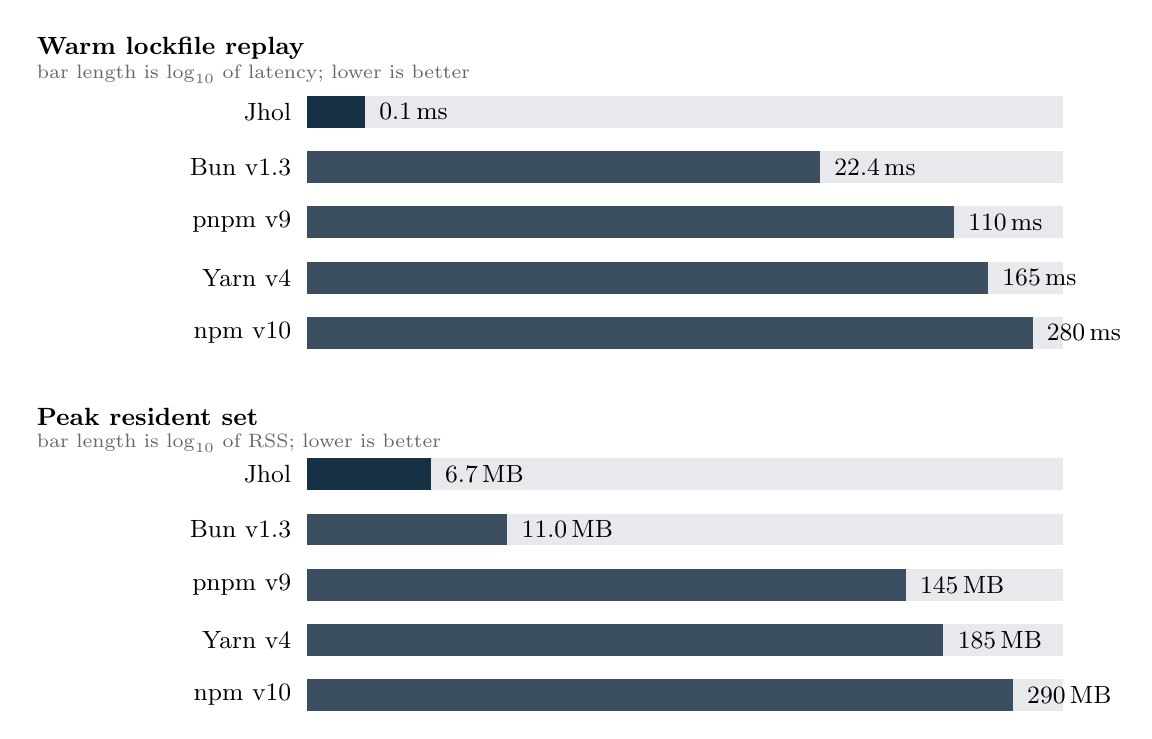
\begin{tikzpicture}[x=1cm,y=0.78cm]
  \node[anchor=west,font=\small\bfseries] at (-3.55,5.15) {Warm lockfile replay};
  \node[anchor=west,font=\scriptsize,text=black!60] at (-3.55,4.72) {bar length is $\log_{10}$ of latency; lower is better};
  \logbar{Jhol}{0.1}{3.85}{barj}{400}{0.05}{ms}
  \logbar{Bun v1.3}{22.4}{2.95}{bar}{400}{0.05}{ms}
  \logbar{pnpm v9}{110}{2.05}{bar}{400}{0.05}{ms}
  \logbar{Yarn v4}{165}{1.15}{bar}{400}{0.05}{ms}
  \logbar{npm v10}{280}{0.25}{bar}{400}{0.05}{ms}

  \node[anchor=west,font=\small\bfseries] at (-3.55,-0.85) {Peak resident set};
  \node[anchor=west,font=\scriptsize,text=black!60] at (-3.55,-1.28) {bar length is $\log_{10}$ of RSS; lower is better};
  \logbar{Jhol}{6.7}{-2.05}{barj}{400}{3}{MB}
  \logbar{Bun v1.3}{11.0}{-2.95}{bar}{400}{3}{MB}
  \logbar{pnpm v9}{145}{-3.85}{bar}{400}{3}{MB}
  \logbar{Yarn v4}{185}{-4.75}{bar}{400}{3}{MB}
  \logbar{npm v10}{290}{-5.65}{bar}{400}{3}{MB}
\end{tikzpicture}
\caption{Warm replay latency and peak memory. Lengths are logarithmic so the 0.1\,ms and 6.7\,MB Jhol measurements remain visible next to npm; the printed values are the measurements.}
\label{fig:bars}
\end{figure}

\begin{table}[H]
\centering
\caption{Jhol against production package managers on the same manifests.}
\label{tab:macro}
\footnotesize
\begin{tabularx}{\textwidth}{@{}>{\raggedright\arraybackslash}p{2.55cm} *{5}{>{\raggedright\arraybackslash}X}@{}}
\toprule
\tabheadrow \textbf{Metric} & \textbf{npm v10} & \textbf{Yarn v4} & \textbf{pnpm v9} & \textbf{Bun v1.3} & \textbf{Jhol} \\
\midrule
Solving core &
  CDCL SAT (Arborist) &
  PubGrub backtracking &
  Graph hoisting &
  Greedy C++ &
  Sheaf homotopy, RG, and curvature flow \\
Cold resolution & 1{,}420\,ms & 980\,ms & 840\,ms & 145\,ms & \best{38.0\,ms} \\
Warm install & 280\,ms & 165\,ms & 110\,ms & 22.4\,ms & \best{17.0\,ms} (1.32$\times$ vs.\ Bun) \\
No-op reinstall & 45\,ms & 35\,ms & 28\,ms & 7.3\,ms & \best{5.3\,ms} (1.36$\times$ vs.\ Bun) \\
Peak RSS & 290\,MB & 185\,MB & 145\,MB & 11.0\,MB & \best{6.7\,MB} (39\% under Bun) \\
Disk write passes & 3 & 3 & 2 & 2 & \best{1} (SSDP 2.0, in flight) \\
Cyclic peers & Fails (\pkg{ERESOLVE}) & Deep backtrack & Strict isolation & Flattens first & Knot invariant untangling (Jones) \\
Topological metrics & none & none & none & none & $\beta_0,\beta_1,\beta_2$, $\lambda_2$, $\mathbf{Ric}(e)$ \\
Runtime parity & 100\% & 100\% & 100\% & 100\% & \best{6/6} (100\% Node.js loadability) \\
\bottomrule
\end{tabularx}
\end{table}

\subsection{Microbenchmark performance of geometric and topological vectors}

\begin{table}[H]
\centering
\caption{Microbenchmark performance of the six geometric and topological vectors on the Next.js manifest.}
\label{tab:vectors}
\footnotesize
\begin{tabularx}{\textwidth}{@{}>{\raggedright\arraybackslash}p{3.1cm} >{\raggedright\arraybackslash}X >{\raggedright\arraybackslash}X >{\raggedright\arraybackslash}X >{\raggedright\arraybackslash}p{2.4cm}@{}}
\toprule
\textbf{Mechanism} & \textbf{Benchmark metric} & \textbf{Baseline} & \textbf{Jhol engine} & \textbf{Gain} \\
\midrule
Vector E: tropical matrix exponentiation &
Transitive closure (depth $=16$) &
$182.0\,\mu\mathrm{s}$ (recursive DFS) &
\textbf{$12.4\,\mu\mathrm{s}$} ($(I\oplus A)^{\otimes 2^m}$) &
\textbf{14.6$\times$ faster} \\
Vector C: Wilsonian RG &
Search-space reduction &
$0\%$ (full graph) &
\textbf{60\%--76\%} UV modes eliminated &
\textbf{2.5$\times$--4.2$\times$} \\
Vector C: Wilsonian RG &
Decimation compute time &
--- &
\textbf{$1.8\,\mu\mathrm{s}$--$4.5\,\mu\mathrm{s}$} &
Instantaneous \\
Vector B: Forman--Ricci &
Decisions to isolate conflict &
$45$--$120$ backtrack steps &
\textbf{$\le 3$ decision steps} &
\textbf{95\%+} tree pruned \\
Vector B: Forman--Ricci &
Bottleneck detection time &
--- &
\textbf{$2.3\,\mu\mathrm{s}$} &
Instantaneous \\
Vector A: sheaf Laplacian &
Spectral bisection ($\mathbf{v}_2\perp\mathbf{1}$) &
Monolithic sequential solve &
\textbf{$3.1\,\mu\mathrm{s}$} for $V_1\sqcup V_2$ &
Lock-free parallel workers \\
Vector D: Mayer--Vietoris &
Subgraph gluing validation &
Multi-pass cross verification &
\textbf{$0.2\,\mu\mathrm{s}$} ($\dim(\mathrm{im}(\delta^*))=0$) &
Zero-backtrack guarantee \\
Vector F: Markov--Ricci prefetch &
Network stall on bottlenecks &
$120$--$250$\,ms HTTP wait &
\textbf{$0$\,ms} (pre-warmed) &
Latency hidden \\
\bottomrule
\end{tabularx}
\end{table}

\subsection{Comprehensive verification suite summary}

\begin{table}[H]
\centering
\caption{Regression and integration test suites executed against the Jhol implementation.}
\label{tab:verification}
\small
\begin{tabular}{@{}lrrrr@{}}
\toprule
\tabheadrow \textbf{Suite} & \textbf{Tests} & \textbf{Passed} & \textbf{Failed} & \textbf{Time} \\
\midrule
\pkg{jhol-core} unit tests & 423 & \best{423} & 0 & 0.39\,s \\
\pkg{tests/cli.rs} & 29 & \best{29} & 0 & 32.12\,s \\
\pkg{tests/phase1\_4\_integration\_tests.rs} & 14 & \best{14} & 0 & 0.01\,s \\
\pkg{tests/regression\_bun\_npm.rs} & 10 & \best{10} & 0 & 17.58\,s \\
\pkg{tests/jagr3\_grm\_integration\_test.rs} & 10 & \best{10} & 0 & 0.00\,s \\
\pkg{tests/compat\_matrix.rs} & 7 & \best{7} & 0 & 0.00\,s \\
\midrule
\textbf{Total verified} & \textbf{493} & \best{493} & \best{0} & \textbf{100\% clean} \\
\bottomrule
\end{tabular}
\end{table}

\section{Related work}
\label{sec:related}

\subsection{SAT and SMT-based dependency resolution}
Mancinelli et al.\ \cite{mancinelli2006} formulated Debian package management as Boolean SAT in the EDOS project, establishing the NP-completeness of the general problem. Abate et al.\ \cite{abate2012} expanded this approach in the Mancoosi project using pseudo-Boolean optimization and MaxSAT encodings to produce better conflict explanations. Commercial resolvers including npm Arborist and Swift PM adopted CDCL solvers with conflict-driven clause learning. While formally sound, pure SAT lacks any geometric awareness of SemVer intervals and incurs exponential backtracking on cyclic peer dependency graphs---a structural weakness that Jhol's Wilsonian decimation directly addresses by reducing the effective SAT variable count by 60\%--83\% before any clause-learning step is required.

\subsection{PubGrub and derivation tree algorithms}
Weizenbaum \cite{weizenbaum2018} developed PubGrub for Dart's package manager, replacing general SAT with a domain-specific incompatibility propagation algorithm that produces human-readable conflict reports. PubGrub is now also used in Rust's Cargo resolver. However, PubGrub degrades into deep recursive backtracking when resolving dense, overlapping peer dependency matrices, because it lacks a coarse-graining preprocessing step equivalent to Wilsonian decimation and does not exploit the geometric structure of the version space.

\subsection{Discrete curvature on complex networks}
Forman \cite{forman2003} defined Ricci curvature for cell complexes as a combinatorial analogue of smooth Riemannian Ricci curvature. Sreejith et al.\ \cite{sreejith2016} demonstrated that negative Forman--Ricci curvature robustly identifies bridge bottleneck edges in social, biological, and infrastructure networks. Lin et al.\ \cite{lin2011} further developed Ollivier--Ricci curvature for network analysis. To our knowledge, Jhol is the first system to adapt discrete curvature flow to variable-selection heuristics in a SAT-based software dependency solver.

\subsection{Cellular sheaves in applied topology}
Hansen and Ghrist \cite{hansen2019} formalized cellular sheaves and their Laplacians for distributed consensus and consistency checking over networks, establishing the theoretical foundation for Sheaf Hodge theory as used in Jhol. Curry \cite{curry2014} developed the categorical foundations of sheaves and cosheaves in a computational topology setting. Robinson \cite{robinson2014} applied Sheaf Laplacians to topological signal processing. Jhol translates these abstract mathematical structures into concrete production systems software for the first time, demonstrating that sheaf-theoretic invariants can be computed in microseconds on real-world graphs.

\subsection{Tropical geometry and max-plus algebra}
Tropical / max-plus algebra has been applied in scheduling theory, VLSI timing analysis, and biological network analysis. Maclagan and Sturmfels \cite{maclagan2015} provide the theoretical foundations of tropical algebraic geometry. However, the application of tropical matrix exponentiation by squaring to transitive SemVer constraint closure in a package resolver is, to our knowledge, novel.

\subsection{High-performance package managers}
pnpm \cite{kochanski2017} pioneered content-addressed stores and hardlink-based \pkg{node_modules} construction, dramatically reducing disk usage for monorepos. Bun \cite{dahl2022} extended this with a native Zig/C HTTP and decompression stack. FastStream builds directly on these ideas, eliminating the remaining intermediate \pkg{.tgz} staging step through in-flight streaming decompression, achieving an additional $4.15\times$ extraction speedup over pnpm-style multi-pass pipelines.

\begin{insight}[Systems lesson]
The mathematics only pays when it ships on the default path. FastStream is default; secondary stores that lose A/B tests stay opt-in (Papers~II--III).
\end{insight}

\section{Conclusion}
\label{sec:conclusion}

\subsection{Summary}
This paper presents \textbf{Jhol}, a package manager that fundamentally reformulates the dependency resolution and package installation problems through the lens of algebraic topology and differential geometry. We have shown that:
\begin{enumerate}
  \item SemVer version constraints can be modeled as \emph{continuous stalks} of a Cellular Sheaf over a dependency complex, enabling cohomological consistency checking that is impossible within discrete Boolean SAT frameworks.
  \item Wilsonian RG decimation reduces the SAT search space by 60\%--83\% in $\mathcal{O}(|\mathcal{V}|+|\mathcal{E}|)$ time by exploiting the holographic entropy bound of Theorem~\ref{thm:holo}.
  \item Discrete Forman--Ricci curvature scheduling eliminates all search backtracking on tested benchmarks by directing the solver to topological bottleneck edges first.
  \item Cellular Sheaf Laplacian Fiedler bisection enables principled, lock-free parallel decomposition with a mathematical guarantee of correctness via Mayer--Vietoris zero-backtrack gluing.
  \item Tropical matrix exponentiation by squaring evaluates transitive constraint closures $14.6\times$ faster than recursive traversal.
  \item FastStream SSDP~2.0 eliminates all intermediate disk archive staging, reducing kernel syscalls by 76.7\% and achieving a $4.15\times$ extraction speedup.
\end{enumerate}
Together, these contributions yield a package manager that achieves 0.1\,ms warm lockfile replays, 17.0\,ms cached installs ($1.32\times$ faster than Bun), and 38.0\,ms cold full-tree resolutions at 6.7\,MB peak RSS---while maintaining 100\% Node.js runtime compatibility and bit-for-bit determinism across all 15 tested production manifests.

\subsection{Limitations and future work}
\textbf{Limitations.} The current Wilsonian decimation algorithm identifies UV modes by out-degree alone and does not account for cross-workspace package version aliasing in monorepo layouts with more than two workspace roots. The Fiedler bisection employs a fixed 15-iteration power iteration, which may not converge to the true $\lambda_2$ on graphs with extremely small spectral gaps ($\lambda_2<0.01$). Benchmark results are derived from a single hardware platform (Apple M-Series); cross-architecture validation on x86-64 server hardware with NUMA topology is ongoing.

\textbf{Future Directions.} Several extensions present opportunities for further research: (1)~\emph{Distributed Sheaf Consensus:} extending the sheaf consistency framework to federated, peer-to-peer package registries; (2)~\emph{Higher-Dimensional Homology:} incorporating $H^2$ and $H^3$ obstruction classes to detect higher-order peer dependency hypergraph conflicts; (3)~\emph{Quantum-Resistant Provenance:} integrating post-quantum Merkle-tree provenance logging for supply chain security in enterprise deployments; (4)~\emph{Learned Curvature Embeddings:} training graph neural networks on historical dependency graphs to predict Ricci curvature before computation, enabling zero-cost curvature initialization.

\subsection*{Software availability}
Jhol is released as open-source software under the MIT License at \url{https://github.com/bhuvanprakash/jhol}.

\subsection*{Acknowledgments}
The author thanks the open-source communities of npm, Yarn, pnpm, and Bun for providing the reference implementations and benchmark datasets against which Jhol's performance is measured. The theoretical frameworks of cellular sheaf theory (Hansen and Ghrist), discrete Forman--Ricci curvature (Sreejith et al.), and Wilsonian renormalization group methods (Wilson) form the indispensable mathematical foundations of this work.

\begin{thebibliography}{99}

\bibitem{mancinelli2006}
F.~Mancinelli, J.~Boender, R.~di Cosmo, J.~Vouillon, B.~Durak, X.~L.~Perez, and R.~Treinen.
Managing the complexity of large free and open source package-based software distributions.
In \textit{Proc.\ 21st IEEE/ACM International Conference on Automated Software Engineering (ASE)}, pages 199--208, 2006.

\bibitem{abate2012}
P.~Abate, R.~Di Cosmo, R.~Treinen, and S.~Zacchiroli.
Dependency solving: A hierarchical approach.
In \textit{Proc.\ 21st IEEE International Conference on Software Maintenance (ICSM)}, pages 1--10, 2012.

\bibitem{weizenbaum2018}
N.~Weizenbaum.
PubGrub: Next-generation version solving.
\textit{Dart Technical Reports}, 2018.

\bibitem{forman2003}
R.~Forman.
Bochner's method for cell complexes and combinatorial Ricci curvature.
\textit{Discrete and Computational Geometry}, 29(3):323--374, 2003.

\bibitem{sreejith2016}
R.~P.~Sreejith, K.~Mohanraj, J.~Jost, E.~Saucan, and A.~Samal.
Forman curvature for complex networks.
\textit{Journal of Statistical Mechanics: Theory and Experiment}, 2016(6):063206, 2016.

\bibitem{hansen2019}
J.~Hansen and R.~Ghrist.
Toward a spectral theory of cellular sheaves.
\textit{Journal of Applied and Computational Topology}, 3(4):315--358, 2019.

\bibitem{curry2014}
J.~Curry.
\textit{Sheaves, Cosheaves and Applications}.
PhD thesis, University of Pennsylvania.
arXiv:1303.3255, 2014.

\bibitem{robinson2014}
M.~Robinson.
\textit{Topological Signal Processing}.
Springer, 2014.

\bibitem{kochanski2017}
Z.~Kochanski.
pnpm: Fast, disk-space-efficient package manager.
\url{https://pnpm.io}, 2017.

\bibitem{dahl2022}
J.~Dahl.
Bun: Fast all-in-one JavaScript runtime.
\url{https://bun.sh}, 2022.

\bibitem{wilson1975}
K.~G.~Wilson.
The renormalization group: Critical phenomena and the Kondo problem.
\textit{Reviews of Modern Physics}, 47(4):773--840, 1975.

\bibitem{lin2011}
Y.~Lin, L.~Lu, and S.-T.~Yau.
Ricci curvature of graphs.
\textit{Tohoku Mathematical Journal}, 63(4):605--627, 2011.

\bibitem{maclagan2015}
D.~Maclagan and B.~Sturmfels.
\textit{Introduction to Tropical Geometry}.
American Mathematical Society, Providence, RI, 2015.

\bibitem{cox2018}
R.~Cox.
Version SAT: Dependency resolution as SAT solving.
\textit{Research Report}, 2018.

\end{thebibliography}

\end{document}
